

%%%%%%%%%%%%%%%%%%%%%%%%%%%%%%%%%%%%%%%%%
% University/School Laboratory Report
% LaTeX Template
% Version 3.1 (25/3/14)
%
% This template has been downloaded from:
% http://www.LaTeXTemplates.com
%
% Original author:
% Linux and Unix Users Group at Virginia Tech Wiki 
% (https://vtluug.org/wiki/Example_LaTeX_chem_lab_report)
%
% License:
% CC BY-NC-SA 3.0 (http://creativecommons.org/licenses/by-nc-sa/3.0/)
%
%%%%%%%%%%%%%%%%%%%%%%%%%%%%%%%%%%%%%%%%%

%----------------------------------------------------------------------------------------
%	PACKAGES AND DOCUMENT CONFIGURATIONS
%----------------------------------------------------------------------------------------

\documentclass{article}

\usepackage[version=3]{mhchem} % Package for chemical equation typesetting
\usepackage{siunitx} % Provides the \SI{}{} and \si{} command for typesetting SI units
\usepackage{graphicx} % Required for the inclusion of images
\usepackage{natbib} % Required to change bibliography style to APA
\usepackage{amsmath} % Required for some math elements 
\usepackage{listings}
\usepackage{color}
\usepackage{caption}
\usepackage{rotating}
\usepackage{enumitem}
\usepackage{url}
%\usepackage{hyperref}

\definecolor{dkgreen}{rgb}{0,0.6,0}
\definecolor{gray}{rgb}{0.5,0.5,0.5}
\definecolor{mauve}{rgb}{0.58,0,0.82}

\lstset{frame=tb,
  language=Java,
  aboveskip=3mm,
  belowskip=3mm,
  showstringspaces=false,
  columns=flexible,
  basicstyle={\small\ttfamily},
  numbers=none,
  numberstyle=\tiny\color{gray},
  keywordstyle=\color{blue},
  commentstyle=\color{dkgreen},
  stringstyle=\color{mauve},
  breaklines=true,
  breakatwhitespace=true,
  tabsize=3
}
\setlength\parindent{0pt} % Removes all indentation from paragraphs

\renewcommand{\labelenumi}{\alph{enumi}.} % Make numbering in the enumerate environment by letter rather than number (e.g. section 6)

%\usepackage{times} % Uncomment to use the Times New Roman font

%----------------------------------------------------s------------------------------------
%	DOCUMENT INFORMATION
%----------------------------------------------------------------------------------------

\title{Laboratory Assignment 6 Write Up \\ Computer Science 441} % Title

\author{\textsc{Andreas Bach Landgrebe}} % Author name

\date{\today} % Date for the report

\begin{document}

\maketitle % Insert the title, author and date

\begin{center}
\begin{tabular}{l r}
Date Submitted:  March 7, 2016 \\ % Date the experiment was performed
Partners:  Andreas Bach Landgrebe  \\ % Partner names
Instructor:  Dr. Gregory M. Kapfhammer  % Instructor/supervisor
\end{tabular}
\end{center}

% If you wish to include an abstract, uncomment the lines below
% \begin{abstract}
% Abstract text
% \end{abstract}

%----------------------------------------------------------------------------------------
%	SECTION 1
%----------------------------------------------------------------------------------------

\section{The well-commented source code of the Java class called MulticastSocketSender.}
\textbf{MulticastSocketSender.java}
\begin{lstlisting}
//import statements
import java.io.IOException;
import java.net.DatagramPacket;
import java.net.DatagramSocket;
import java.net.InetAddress;
import java.net.UnknownHostException;

public class MulticastSocketSender {

  // This example is from: http://examples.javacodegeeks.com/core-java/net/multicastsocket-net/java-net-multicastsocket-example/

  final static String INET_ADDR = "224.0.0.3";
  //This is the IP address tht you are going to connect to hopefully
  final static int PORT = 12345;
  //This is the port nuymber being used to perform this communication

  public static void main(String[] args) throws UnknownHostException, InterruptedException {
    // Get the address that we are going to connect to.
    InetAddress addr = InetAddress.getByName(INET_ADDR);

    // Open a new DatagramSocket, which will be used to send the data.
    try (DatagramSocket serverSocket = new DatagramSocket()) {
      for (int i = 0; i < 5; i++) {
        //try to connect to the receiver and the message is just the number 0 to 4.
        String msg = "Sent message number: " + i;
        //this is the string or message being sent

        // Create a packet that will contain the data
        // (in the form of bytes) and send it.
        DatagramPacket msgPacket = new DatagramPacket(msg.getBytes(),
            msg.getBytes().length, addr, PORT);
        //send the packet that is the object DatagramSocket 
        serverSocket.send(msgPacket);

        System.out.println("The server sent a packet with this message: " + msg);
        //print the message


        Thread.sleep(500);
        //this line suspends the thread from doing its thing for a period of time.
        //in this case, it is 500 milliseconds
      }
    } catch (IOException ex) { //if the connection is not successful, then catch it.
      ex.printStackTrace();
    }
  }
}

\end{lstlisting}
%----------------------------------------------------------------------------------------
%	SECTION 2
%----------------------------------------------------------------------------------------

\section{The well-commented source code of the Java class called MulticastSocketReceiver.}
\textbf{MulticastSocketReceiver.java}
\begin{lstlisting}
//import statements
import java.io.IOException;
import java.net.DatagramPacket;
import java.net.InetAddress;
import java.net.MulticastSocket;
import java.net.UnknownHostException;

public class MulticastSocketReceiver {

  // This example is from: http://examples.javacodegeeks.com/core-java/net/multicastsocket-net/java-net-multicastsocket-example/

  final static String INET_ADDR = "224.0.0.3";
  //This is the IP address that you are going to connect to hopefully
  final static int PORT = 12345;
  //This is the port number being used to perform this communication.
  public static void main(String[] args) throws UnknownHostException {
    // Get the address that we are going to connect to.
    InetAddress address = InetAddress.getByName(INET_ADDR);

    // Create a buffer of bytes, which will be used to store
    // the incoming bytes containing the information from the server.
    // Since the message is small here, 256 bytes should be enough.
    byte[] buf = new byte[256];

    // Create a new Multicast socket (that will allow other sockets/programs
    // to join it as well.
    try (MulticastSocket clientSocket = new MulticastSocket(PORT)){
      //try to connect using the multi cast socket

      //Joint the Multicast group.
      clientSocket.joinGroup(address);


      while (true) {
        // Receive the information and print it.
        DatagramPacket msgPacket = new DatagramPacket(buf, buf.length);  
        clientSocket.receive(msgPacket);

        String msg = new String(buf, 0, buf.length);

        System.out.println("The socket received this message: " + msg);
        //this message will print out while the connection is still active
      }
    } catch (IOException ex) { //catch the exception if the connection is not successful
      ex.printStackTrace();
    }
  }
}
\end{lstlisting}

%----------------------------------------------------------------------------------------
%	SECTION 3
%----------------------------------------------------------------------------------------
\section{Using both text and diagrams, a description of the client-server communication with multicasting.}

It is important to be able to know how the client-server communication works with multicasting. To best describe this communication, the diagram below best describes the interaction between the client and the server with performing multicasting.

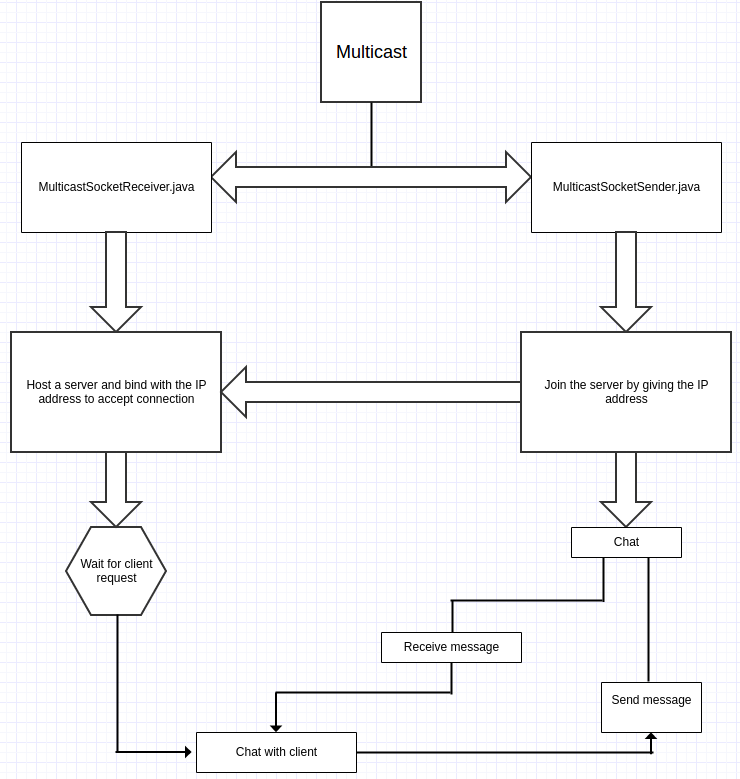
\includegraphics[scale=0.5]{csmulticast.png}

In order to have this program for this laboratory assignment to work properly, the first thing that needs to occur is the MulticastSocketReceiver.java needs to run. After the MulticastSocketReceiver.java runs, then one is able to run the MulticastSocketSender. This is due to the fact that the Sender will not know who is receiving. After the receiver runs first and then the sender, the next thing that occurs has something to do with IP address. On the sender side, the sender will join the server or the receiver by giving the IP address. For this laboratory assignment, the IP address that is being used is 224.0.0.3. This IP address is in the range of multicast addresses. Multicast addresses are in the range 224.0.0.0 to 239.255.255.255. After the sender join the receiver by giving the IP address (224.0.0.3), the server or receiver will host a server and bind with the IP address to accept the connection. If the sender and the receiver do not operate on the same IP address, then this connection will not work properly so it is important that the client and the server operate on the same IP address. After the connection has been accepted, the receiver will wait for the client or sender request. For this laboratory assignment, the messages that is being sent is the number 0, 1, 2, 3, and 4 being performed in a for loop.  

%----------------------------------------------------------------------------------------
%	SECTION 4
%----------------------------------------------------------------------------------------

\section{A report that explicitly compares and contrasts multicast and unicast remote communication.}

There are quite a few differences between multicast and unicast remote communication. A unicast communication is used when two network nodes need to work with each other. This association is considered to be one to one. This is different when it comes to multicast. The association with multicast is considered to be one to many nodes. The intent of multicasting is to have a sender send to multiple network nodes or a particular group of hosts on a network segment. There are a few examples of multicast and unicast communication in Internet Protocol version 4 (IPv4). One example of using a unicast communication in IPv4 is browsing the internet. An example of a multicast communication in IPv4 is Internet Protocol television (IPTV). IPTV is a system where TV services are being delivered using a Internet Protocol. A services being provided by IPTV could be Video on demand (VOD). VOD is where one could browse a catalog of video which is not related to TV programming. There is only one similarity that comes to mind when looking at the unicast and multicast communication. This is when the sender or client is sending information to the receiver or server. There is always one network node for the client or sender. 
%----------------------------------------------------------------------------------------
%	SECTION 5
%----------------------------------------------------------------------------------------
\section{A document that summarizes the different types of multicasting systems used in production.}

There are several systems used in production and real world software that use multicasting. When considering the core of the network, in order to make the most efficient use of network bandwidth, Internet Protocol (IP) multicasting is used for wide area networking \cite{Dutta:2002:MSS:570705.570717}.  Because of multicasting, systems such as TV networks and Internet radios are able to succeed. This is due to the fact that in order to approach the challenge of the use of the network bandwidth to be used the efficient way, the best way to do this is by having the servers of receivers listen by a particular group of hosts on a network segment. One major benefit of using multicasting is that when looking into video ffed, it will not use a massive amount of bandwidth on the part of the server that is delivering. Another system used in production that uses multicasting is HP printers. This is the case so that when one is on a network. it makes it much easier to learh what printers was available. Another multicasting system used in production are electronic exchanges like NASDAQ (National Association of Securities Dealers Automated Quotations \citep{2001:IMS:380749.380771}. Systems like this have to use multicasting because there are a large number of receivers that should receive the same information simultaneously \citep{2001:IMS:380749.380771}.


%----------------------------------------------------------------------------------------
%	SECTION 6
%----------------------------------------------------------------------------------------
\section{A paper that responds to the other questions that this assignment poses about multicasting.}

%What are the key aspects of how these two Java classes support multicast communication

\begin{enumerate}
\item What are the key aspects of how these two Java classes support multicast communication?

The key aspects of the Java classes that support multicast communication is the use of the Java classes java.net.DatagramPacket, java,net.InetAddress, and java.net.MulticastSocket. The purpose of the java.net.DatagramPacket java class is to be able to represent a socket for sending and receiving datagram packets \cite{atagramsocket_java_platform_se_7}. The purpose of the java.net.InetAddress java class is to be able to represent an IP address \cite{inetaddress_java_platform_se_6}. The purpose of the java.net.MulticastSocket is to be able to send and recieve IP multicast packets. This MulticastSocket is a DatagramSocket with additional capabilities for joining several multicast hosts on the Internet \cite{multicastsocket_java_platform_se_7_b12}.

\item In the paper ``An Internet Multicast System for the Stock Market", how is the approach to multicasting that this paper presents different than the one that you have used in this laboratory assignment?

The paper's approach to multicateing is different than the one we had used in the laboratory assignment by the fact that in the laboratory assignment, there was a default IP address being used so the client or sender and server or receiver was able to communicate with each other. The approach in the paper will be using multiple IP address for differnet purposes.

\item Would it be a good idea to use the code from this laboratory assignment in a multisystem for the stock market? Why or why not?

No, in fact, it would be a horrible idea to use the code from this laboratory assignment in a multisystem for the stock market. The reason for my answer is because in the laboratory assignment, we were only using one IP address to perform multicasting.In our source code, it was hard coded to only use one IP address. In the stock market, they would need to be able to access to multiple IP address to ensure that all traders and other receivers receive the same information at the same time. If it was the case that we used our source code for the stock market, then we would only have one IP address to use and the system will crash on multiple occasions. One would need to re-write the code to ensure that multiple IP address are being used that a system so big like a stock market does not crash.
\end{enumerate}

%Can you draw a technical diagram that illustrates the general interaction between a client and a server, customized for these two classes that perform multicast communication with sockets?

% "An Internet multicast system for the stock market"
% - How is the approach to multicasting that this paper presents different than the one that you have used in this laboratory assignment?
% - Would it be a good idea to use the code from this laboratory assignment in a multicasting system for the stock market? NO
% 

%----------------------------------------------------------------------------------------
% SECTION 7
%----------------------------------------------------------------------------------------
\section{A reflection on the challenges that you encountered when completing this assignment.}

There was one main that I had encountered when completing this assignment. This challenge was completing the laboratory assignment on my MacBook Pro using Mac OS X. When I was trying to run the given source code on my Mac OS X, I as receiving a java.net.SocketException error on the MulticastSocketReceiver. This was due to the fact that the Mac OS X operating system did not get a default network interface from the IPv6 address. To overcome this issue, I decided to use the Ubuntu operating system that I had on my other machines that I own. 

%----------------------------------------------------------------------------------------
%	BIBLIOGRAPHY
%----------------------------------------------------------------------------------------

\nocite{tanenbaum_steen_2007}
\nocite{2001:IMS:380749.380771}
\nocite{Dutta:2002:MSS:570705.570717}
\nocite{datagramsocket_java_platform_se_7}
\nocite{inetaddress_java_platform_se_6}
\nocite{multicastsocket_java_platform_se_7_b123}
\bibliographystyle{plain}
%\bibliographystyle{IEEEtran}
\bibliography{sample}

%----------------------------------------------------------------------------------------


\end{document}
